% !TEX root = ../Thesis.tex
\chapter{Implementation}

In this section, we will introduce how we implemented a word-gesture keyboard using Unity, a python script and the $\text{SHARK}^2$ system.

\section{Word Graph Generator}
As mentioned in the background section, in the part about $\text{SHARK}^2$ (\ref{SHARK2}), to make $\text{SHARK}^2$ work, the perfect graphs for all the words in a lexicon are needed to be precalculated. Therefore, we needed a script, that either creates or overwrites a file for every available keyboard layout. It has to write the words included in the lexicon together with the corresponding $N$ sampled points of every graph in it. Such a file contains per line a word, then a certain number of points from the word's perfect graph followed by the same points, but normalized (normalized as mentioned in the background section about $\text{SHARK}^2$ (\ref{normalize}))\\
To run the script, the user has to provide the name of the layout that they want to create the perfect graphs for. Additionally, they also have to write the name of the text file containing all the words (lexicon). The script then either creates a new file named ``sokgraph\_\textit{layout}.txt'' or if already a file with this name exists, it deletes its content. Then it fills the file line by line as mentioned above.\\
The file can only be executed for one layout at a time. Hence, if there are more available layouts for our word-gesture keyboard, the user has to run the script for every single one, which can take a bit of time. To calculate and write a file for all about 10'000 words in our used lexicon, it takes about four to five seconds.\\
One thing the script pays attention to is, if a word can be written with used layout. If there are words in the lexicon, that can not be written with the given layout, the script skips this one. Hence, there will be no line in the file for said word. 

\section{Used Algorithm}
For our word-gesture keyboard we used a weaker version of the algorithm used in $\text{SHARK}^2$. This means, we do also work with two core channels, a location recognizer and a shape recognizer, but did not implement everything else as they did in $\text{SHARK}^2$. The shape recognizer is to calculate the deviation from the user inputted graph and a perfect graph from a word with respect to their shape. The location recognizer is for the same thing, but not with respect to the shape, but rather the position on the keyboard. When looking at the shape, we have to normalize the graphs in a specific way (as mentioned in section (\ref{normalize})), so the position, where they exactly lie on the keyboard, does not matter. When looking at the location, we look at the graphs as they are, without normalizing or changing anything.\\
As in the $\text{SHARK}^2$ system we also use the start and end positions of the graphs as a first pruning method. The difference is, that for $\text{SHARK}^2$, the authors chose to normalize all the graphs in scale and translation before comparing the start-to-start and end-to-end positions. In our algorithm, we do not normalize the graphs, but just look at the start and end positions of a user input graph and a word's graph. As threshold we set the width of a key. That means, if either the start-to-start or end-to-end position is bigger than a key width, the word to which this applies, gets discarded.\\
Another thing we implemented differently is $\sigma$. For the channel integration formula \ref{eqn:gaussian}, they used $\sigma$ in $\text{SHARK}^2$ as a parameter. They determine its value by the gesturing speed (\ref{gesturing speed}). We do not use the gesturing speed in our algorithm. For the location channel (in the formula \ref{eqn:gaussian}) we use as fixed value for $\sigma$ the radius of a key TODO: IS IT WIDTH OR RADIUS?. For the shape channel (in the formula \ref{eqn:gaussian}) we use a variable value. We take a value that equals the radius of a normalized key. That means, a small graph will have a bigger $\sigma$ than a big graph, because we do normalize the graphs longer bounding box' side to a fixed length. Therefore, a small graph gets stretched by it, whereby a big graph gets contracted.\\
As mentioned in the beginning of this section, we use a weaker form of the algorithm used in $\text{SHARK}^2$. That being said, we do currently not use any language information nor dynamic channel weighting by gesturing speed. We do not user any language information, because that would have gone beyond the scope of this project. The dynamic channel integration was not implemented by us, because in our opinion the value of sigma, as we chose it, is fine for the purpose of our word-gesture keyboard.

\section{Functions}
In this section, we will present the functions our word-gesture keyboard provides.
\begin{figure}
\centering
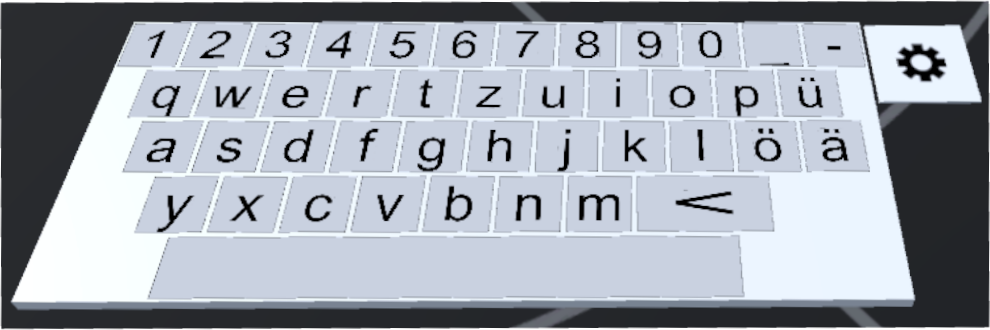
\includegraphics[width=0.7\textwidth]{WGKnormal}
\caption{Word-gesture keyboard in its ``normal'' form without anything selected}
%\label{fig:machine}
\end{figure}
    
\subsection{Text input}
There should be two text input methods for the user. One is the input of words with gestures, the other one is the input of single characters by tapping single keys.

\begin{figure}
\centering
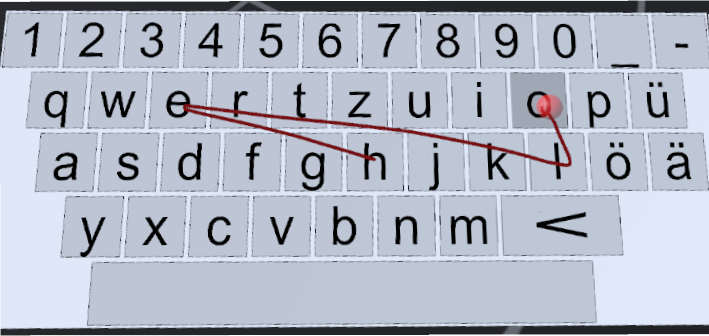
\includegraphics[width=0.4\textwidth]{WGKwrite}
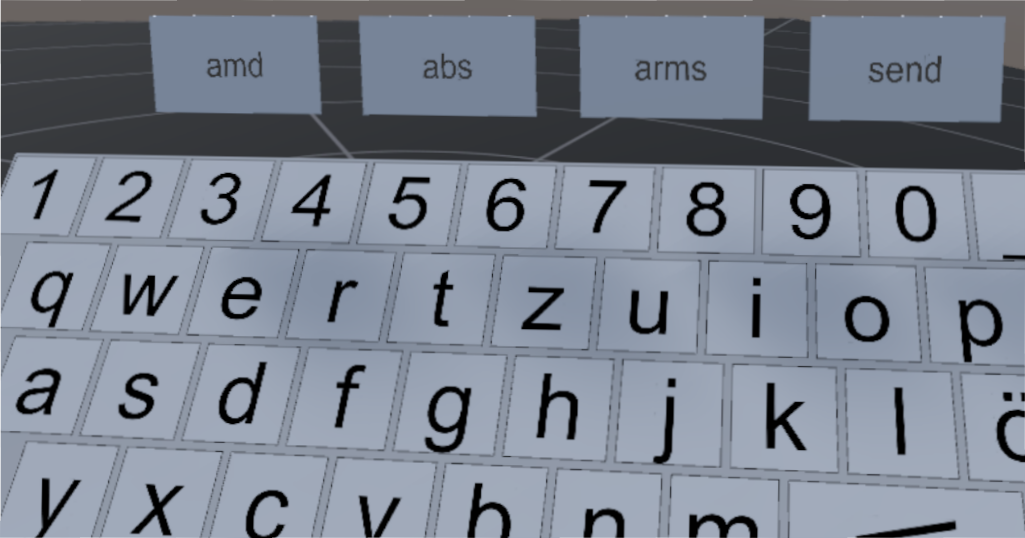
\includegraphics[width=0.4\textwidth]{WGKsuggestions}
\caption{left: the user writes the word ``hello'' as gesture, right: user gets recommended words for ``and''}
\label{fig:write_suggestions}
\end{figure}

\subsubsection{With Gestures}
The most important function our word-gesture keyboard provides, is the writing of words with gestures. A user can press and hold the trigger button of a VR controller inside the keyboard's hitbox and start making a gesture on it. The user will see a red line, that is drawn on the keyboard where they move. This helps them to keep track of the line they drew. When the user wants to finish the gesture, they need to release the trigger of the controller. At this moment, our program starts to evaluate the 5 words with the best match to the user inputted graph. The one with the highest confidence score will be written into the text field. The other 4 are displayed at the keyboard (fig \ref{fig:write_suggestions} right), such that the user can also choose between them. When the user chooses one of these 4 words, the word that has been written into the text field before, is getting replaced by the chosen word and the key, where the chosen word was written, will then display the replaced word.
\subsubsection{As Single Characters}
If the wanted word is not in the lexicon, there will not be any entry in the ``sokgraph\_\textit{layout}.txt''. Therefore, our algorithm will not be able to get this wanted word as best match, hence it can not be written as gesture. For this case, we need a method to input single characters. Fortunately with our word-gesture keyboard this almost works without additional work. If the single letters are as graphs in the layout files, TODO: DEFINE LAYOUT FILES AS SOKRAPH\_LAYOUT.TXT SOMEWHERE. the user is more or less able to write single letters with a gesture. This ``gesture'' would just be a point on the right key, hence a single click at the right position. But there might be a little inconvenience. This is caused by the fact, that we work with distances. The distance from one letter to another is not too big. And if for example the user wants to write an ``e'' but presses the key with the ``e'' on it on its left side and not perfectly in the middle, our system would also evaluate that aside from ``e'', also ``w'' and ``we'' are words, the user might have intended to write (on a conventional qwertz or qwerty layout). To get rid of this, our system checks, if the user inputted graph's bounding box is smaller than TODO: HOW MUCH SMALLER?. It recognizes, that the user wants to write a single letter, and then takes the best match. To get back to the example, ``we'' would be discarded and ``e'' would get a higher score than ``w'', because of a smaller location channel distance. Therefore, the written ``word'' in this case would be ``e''.

\subsection{Create New Layouts}
Another function is the creation of own layouts. A layout text file exists, that contains all available layouts. The user can create as many new layouts as they want to. To create a new one, the user has to write the new layout's name on the first new line. On the following lines they have to write the characters in an order, in which they want to have them on the keyboard. All the unicode characters should be working, but two. In the current implementation, one whitespace is used to declare the position of the spacebar and the ``$<$'' character is used for the backspace key. The layout text file gets read at the start of the program, so it cannot be edited while the program is running, or to be precise, the changes will not be recognized during runtime. One smaller thing we implemented is, that at the start of the program all characters used in the layouts not yet in the lexicon text file and ``sokgraph\_\textit{layout}.txt'' are being added. Without doing this, the user might not be able to input some single characters with their newly created keyboard, because the system simply would not find them in the ``sokgraph\_\textit{layout}.txt'' file. During the runtime, the user then is able to switch between available layouts.

\subsection{Options}

\begin{figure}
\centering
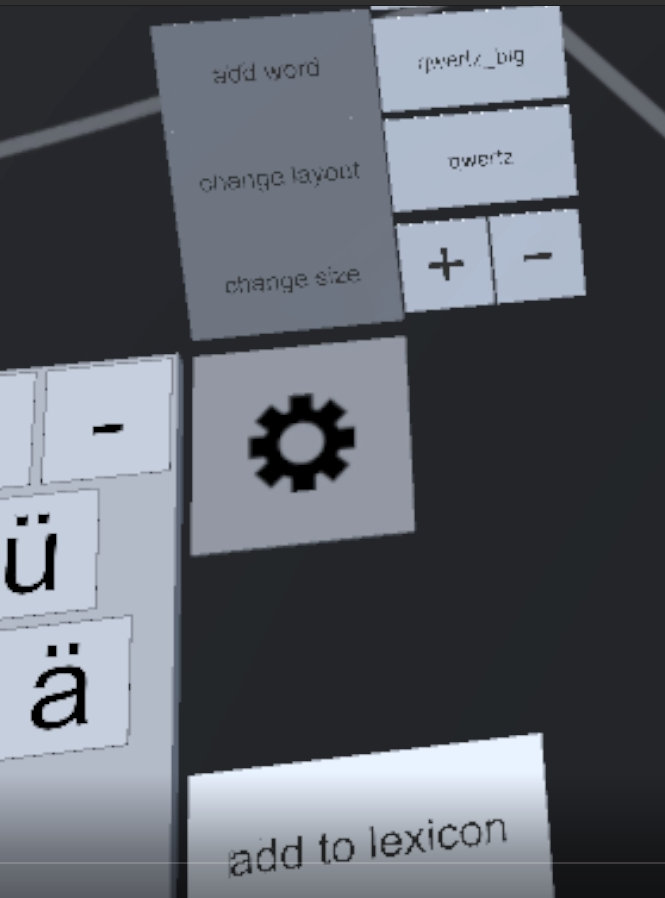
\includegraphics[width=0.4\textwidth]{WGKoptions}
\caption{The options button with all the sub-buttons activated}
%\label{fig:machine}
\end{figure}

To let the user use the other functions, we implemented an options button for our keyboard. It is marked with a black gear. The user can click on it with the trigger button of the controller, when being in the hitbox of it. Then, three new buttons appear each for one currently available option. One is to add new words, one to change the currently selected layout and the last one to scale the keyboard.

\subsubsection{Add Words}
\begin{figure}
    \centering
    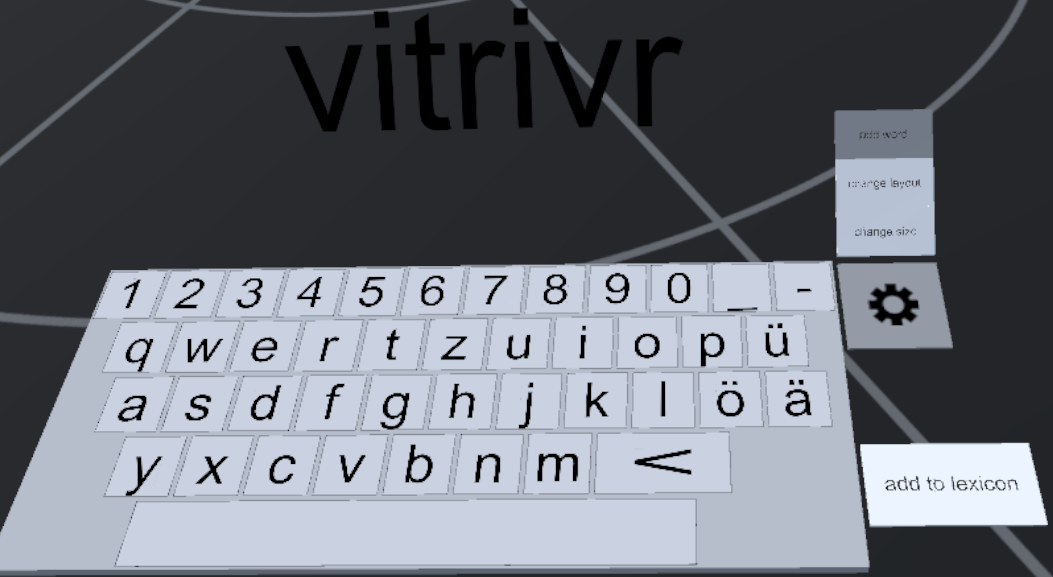
\includegraphics[width=0.4\textwidth]{WGKaddword}
    \caption{``vitrivr'' written with single character inputs, can now be added to the lexicon}
    \label{fig:addword}
    %\label{fig:machine}
\end{figure}
Because the whole system works with a lexicon full of words and only these can be written as gestures, there will also be words the user wants to write, that are not yet in said lexicon. For this case, we implemented a function such that the user can add new words. They can access it via the options button. Then they have to press the button where it says ``add word''. When this button is pressed another button appears, the ``add to lexicon'' button. Now, the user has to input their intended word with single characters. It will be displayed as seen in fig \ref{fig:addword}. Then, when they press the ``add to lexicon'' button, this displayed word will be added to the lexicon text file, if it does not already exist, and does not have a space in it. Additionally, for every available layout, the corresponding graph for the newly added word will also be added to the corresponding ``sokgraph\_\textit{layout}.txt'' text file, such that the user can right after adding the word, write it as gesture. One additional thing we implemented is, that the word's graph only gets appended in the text file, if this word can be written with the layout the file corresponds to. For example, if a user wants to add the word ``öffentlich'', but they made a layout without the letter ``ö'', this word could never be written with said layout, hence it would be unnecessary to have this word in said ``sokgraph\_\textit{layout}.txt'' text file.

\subsubsection{Change Scale and Layout}
There are two other functions that can be found under the options. One is to change the size of the keyboard. When the user clicks on the ``change layout'' button, a ``+'' and a ``-'' button appear. By pressing the ``+'' button, the keyboard gets bigger, by pressing the ``-'' button, the keyboard gets smaller. This can help the user to make the keyboard more handy for them. Depending on how they want to move their arm, they can make it slightly bigger or smaller. If it is bigger, the gestures can be made more precise, if it is smaller, gestures can be made faster.\\
The other function is the ability to change the layout. The user gets a list of all available layouts, when pressing the ``change layout'' button. They then can click on one of these layouts and the keyboard will change its appearance. The available layouts consist of the predefined ones and also of the newly added ones from the user.

\subsection{Other}
TODO: DELETION OF WHOLE WORDS + SPACE INPUT
To end the implementation part, we will shortly talk about the last function, the ability to grab and move the keyboard. This means, the user can grab the keyboard, by being in its hitbox and pressing the controller's grip button. They can move it around in the room and rotate it as they want. We were able to do this thanks to a script that already existed in vitrivr TODO: HOW TO REFERENCE THIS? and did not have to implement anything on our own.